\section{Lecture 7}
\subsection{Lecture Notes - Symmetries and Conservation Laws}
\subsubsection{Noether's Theorem}
Idea: Certain symmetries we observe in nature are associated with conservation laws. E.g. momentum with translational symmetry. Formally, we consider the following:
\newline Consider a Lagrangian $\LL(q, \dot{q}, t)$ is invariant under a coordinate transformation $(q_1, \cdots, q_n) \rightarrow (\tilde{q}_1(\alpha), \cdots, \tilde{q}_n(\alpha))$ with $\tilde{q}_i(\alpha) = q_i + \alpha h_i(q,t) + \delta(\alpha^2)$. Consider taking the derivative with respect to $\alpha$ and set $\alpha = 0$:
\[\left.\dod{}{\alpha}\LL(\tilde{q}(\alpha), \dot{\tilde{q}}(\alpha), t)\right|_{\alpha = 0} = 0\]
Where the expression is zero as $\LL$ is invariant of $\alpha$. Now, by the chain rule, we can say:
\[0 = \left. \sum_{j=1}^n\left(\dpd{\LL}{\tilde{q}_j}\dpd{\tilde{q}_j}{\alpha} + \dpd{\LL}{\dot{\tilde{q}}_j}\dpd{\dot{\tilde{q}}_j}{\alpha}\right)\right|_{\alpha=0}\]
Now, we can say that $\dpd{\dot{\tilde{q}}_j}{\alpha} = \dod{}{t}\dpd{\tilde{q}_j}{\alpha}$ my equality of mixed partials. Using the EL equations, we can also say that $\dpd{\LL}{\tilde{q}_j} = \dod{}{t}\dpd{\LL}{\dot{\tilde{q}}_j}$. We can then write the whole expression as:
\[0 = \left.\dod{}{t}\sum_{j=1}^n\left(\dpd{\LL}{\dot{\tilde{q}}_j}\dpd{\tilde{q}_j}{\alpha}\right)\right|_{\alpha=0}\]
By the chain rule. We have just recollapsed the sum using the chain rule multiple times. Now, call this sum $I(q, \dot{q}, t)$. This object is conserved as its time derivative is zero, i.e. $\dod{}{t}I(q, \dot{q}, t) = 0$. Let us apply this to make this more concrete. 
\subsubsection{Translational and Rotational Symmetry}
Suppose our Lagrangian is $\LL=\frac12 \sum_j m_j \dot{\v{r}}_j^2-U$.
The first symmetry we will consider is the homoegeneity of space. This can be mathematically represented as $\v{r}_i \mapsto \tilde{\v{r}}_i + \alpha\ehat$ (where $\ehat$ is some unit vector) and where $\dot{\v{r}}_i = \dot{\tilde{\v{r}}}_i$. 
\newline The next symmetry we can consider is the isotropy of space. This is represented as $\v{r}_i \mapsto \tilde{\v{r}}_i = \v{r}_i + \hat{\bm{\alpha}}\times \v{r}_i$ (where $\hat{\bm{\alpha}}$ is the axis of rotation).
\begin{center}
    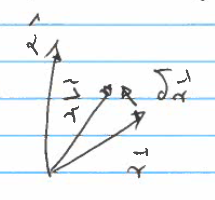
\includegraphics[scale=0.4]{Lecture-7/L7-img1.png}
\end{center}
Now, what does Noether tell us about these symmetries? Assuming that the Lagrangians are invariant under the transformations, then $I$ is conserved, and hence:
\[I = \left.\sum_{j=1}^n\left(\dpd{\LL}{\dot{\tilde{q}}_j}\dpd{\tilde{q}_j}{\alpha}\right)\right|_{\alpha=0} = \begin{cases}
\text{(Translation) } \sum_{j=1}^n m_j\dot{\v{r}}_j \cdot \ehat
\\ \text{(Rotation) } \sum_{j=1}^n m_j\dot{\v{r}}_j \cdot \left(\hat{\bm{\alpha}} \times \v{r}_j\right) = \hat{\bm{\alpha}}\cdot\sum_{j=1}^n \v{r}_j \times m_j \dot{\v{r}}_j
= \hat{\bm{\alpha}}\cdot\v{L}\end{cases}\]
(For rotation, recall that $\v{a}\cdot(\v{b}\times\v{c})=\v{b}\cdot(\v{c}\times\v{a})$.)
In the first case (with translational symmetry) we have conservation of linear momentum along $\ehat$. In the second case (with rotational symmetry) we have the conservation of angular momentum along $\hat{\bm{\alpha}}$.
\subsubsection{Time Symmetry and the Hamiltonian}
We next consider a scenario where we have homogeneity of time; In other words, where $\LL$ is unchanged by $t$. $t \mapsto t + \e$, and $\dpd{\LL}{t} = 0$. Expanding out the total time derivative of the Lagrangian, we have:
\[\dod{}{t}\LL(q, \dot{q}, t) = \sum_{j=1}^n \left(\dpd{\LL}{q_j}\dpd{q_j}{t} + \dpd{\LL}{\dot{q}_j}\dpd{}{t}\dpd{q_j}{t}\right)\]
We recall that $\dpd{q_j}{t} = \dot{q}_j$, $\dpd{\LL}{\dot{q}_j} = p_j$ (generalized momentum) and $\dpd{\LL}{q_j} = \dod{}{t}\dpd{\LL}{\dot{q}_j}$ (generalized force/time derivative of generalized momentum). Again by taking out the time differential operator (by product rule) out of the sum, we have:
\[\dod{}{t}\LL(q, \dot{q}, t) = \dod{}{t}\sum_jp_j\dot{q}_j\]
where $p_j$ is the generalized momentum of the coordinate $q_j$. We can write this as:
\[\dod{}{t}\left(\sum_jp_j\dot{q}_j - \LL\right) = 0\]
And we call the term in the brakets to be the \textbf{Hamiltonian}:
\[\HH = \sum_jp_j\dot{q}_j - \LL\]
which is a conserved quantity.
\subsubsection{Remarks on Hamiltonian}
Hamiltonian is not always conserved $\dod{\HH}{t}\ne0$. It happens when Lagrangian explicitly depends on time. For example, consider a pendulum of length $l$ and blob of mass $m$ subjected to gravity with its attachment point moving at constant angular velocity $\omega$ on a circle of radius $R$.
\begin{center}
    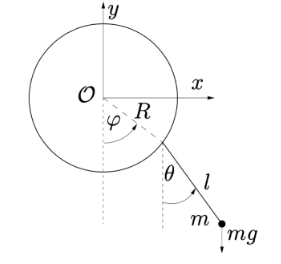
\includegraphics[scale=0.8]{Lecture-7/L7-img2.png}
\end{center}
The Lagrangian for this system is (derivation is left as an exercise):
\[ \LL=\frac{m}{2}\left[ R^2\omega^2+l^2\dot{\theta}^2+2R\omega l \dot{\theta}\cos(\omega t - \theta) \right] + mg(R\cos(\omega t)+l\cos\theta) \]
Since it depends on time, Hamiltonian is not conserved. \\
Hamiltonian of a system is equal to the system's total energy if coordinates are natural (ie. no time dependence):
\[\v{r}_i=\v{r}_i(q_1,q_2,\dots,q_n)\]
Textbook example 7.6 (bead on spinning hoop) is one of the physical situations when Hamiltonian is not equal to the total energy. The coordinate for the bead is:
\[\v{r}=(R\sin\theta\cos(\omega t),R\sin\theta\sin(\omega t),-R\cos\theta)\]
Since it depends on time, the Hamiltonian is not equal to the total energy.